\documentclass[12pt]{article}
\usepackage[utf8]{inputenc}
\usepackage{graphicx}
\usepackage{hyperref}
\usepackage{listings}
\usepackage{xcolor}
\usepackage{geometry}
\usepackage{enumitem}
\usepackage{longtable}
\usepackage{booktabs}
\usepackage[T1]{fontenc}
\usepackage{tikz}
\usetikzlibrary{shapes.geometric, arrows.meta, positioning, fit, calc, backgrounds}
\usepackage{array}

\geometry{a4paper, margin=1in}
\setlength{\emergencystretch}{5em}
\hbadness=5000
\raggedbottom

\renewcommand{\topfraction}{0.9}
\renewcommand{\bottomfraction}{0.9}
\renewcommand{\textfraction}{0.1}
\renewcommand{\floatpagefraction}{0.7}

\makeatletter
\g@addto@macro{\UrlBreaks}{\UrlOrds}
\makeatother

\hypersetup{
    colorlinks=true,
    linkcolor=blue!70!black,
    urlcolor=blue!60!black,
    citecolor=blue!70!black
}

\lstset{
    basicstyle=\ttfamily\footnotesize,
    breaklines=true,
    frame=single,
    numbers=none,
    keywordstyle=\color{blue!70!black},
    commentstyle=\color{green!50!black},
    stringstyle=\color{red!70!black},
    showstringspaces=false,
    tabsize=2,
    backgroundcolor=\color{gray!5}
}

\title{orthodox.net Platform Overview\\[0.5em]\large St.\ Nicholas Orthodox Church\\[0.3em]\small Technical Architecture Summary}
\author{}
\date{March 2026}

\begin{document}

\maketitle

\begin{abstract}
This document provides a high-level technical overview of the orthodox.net platform --- the website of St.\ Nicholas Orthodox Church in McKinney, Texas. The platform consists of two repositories: a quasi-static frontend (\texttt{onet-v2}) deployed on a LAMP stack, and a Python Flask backend API (\texttt{onet-flask-backend}) deployed on Render.com. This overview describes how the components fit together, summarizes the technology stack and external service integrations, and provides pointers to the detailed technical references for each component. It is intended for stakeholders, new team members, or anyone needing a quick understanding of the system without implementation-level detail.
\end{abstract}

\tableofcontents
\newpage

%% ============================================================
\section{Introduction}
%% ============================================================

\subsection{Background}

The original orthodox.net website was built in the early 2000s as a traditional LAMP stack (Linux, Apache, MySQL, PHP) site. Over two decades it accumulated thousands of static HTML pages --- sermons, articles, scripture readings, catechism materials, saints' lives, and more --- many authored in Microsoft Word and exported to HTML.

The \textbf{onet-v2 project} was initiated to modernize the site while keeping it on the same hosting provider (Inoa/Orthodox Internet Services) and progressively replacing legacy pages without modifying them.

\subsection{Repositories}

The platform spans two GitHub repositories:

\begin{longtable}{p{4cm}p{8.5cm}}
\toprule
\textbf{Repository} & \textbf{Purpose} \\
\midrule
\texttt{onet-v2} \newline \url{https://github.com/GZancewicz/onet-v2} & Frontend: HTML, CSS, JavaScript, PHP fetcher scripts, Apache configuration, Python utilities. Deployed on Inoa shared hosting. \\
\midrule
\texttt{onet-flask-backend} \newline \url{https://github.com/GZancewicz/onet-flask-backend} & Backend API: Python Flask REST API aggregating content from Ghost CMS, YouTube, and Google Calendar. Deployed on Render.com. \\
\bottomrule
\end{longtable}

\subsection{Detailed References}

Each repository has its own in-depth technical reference document:

\begin{itemize}
    \item \textbf{Frontend}: \texttt{onet-v2/doc/latex/onet\_frontend/onet\_frontend.pdf} (36 pages) --- covers production server architecture, Apache routing, legacy migration system, JavaScript architecture, deployment, and troubleshooting.
    \item \textbf{Backend}: \texttt{onet-flask-backend/doc/latex/onet\_backend/onet\_backend.pdf} --- covers API endpoints, database schema, caching strategy, Render.com deployment, and module internals.
\end{itemize}

This overview document intentionally avoids duplicating their content. It focuses on how the pieces fit together.

%% ============================================================
\section{System Architecture}
%% ============================================================

Figure~\ref{fig:platform-arch} shows the complete platform architecture.

\begin{figure}[ht]
\centering
\resizebox{\textwidth}{!}{%
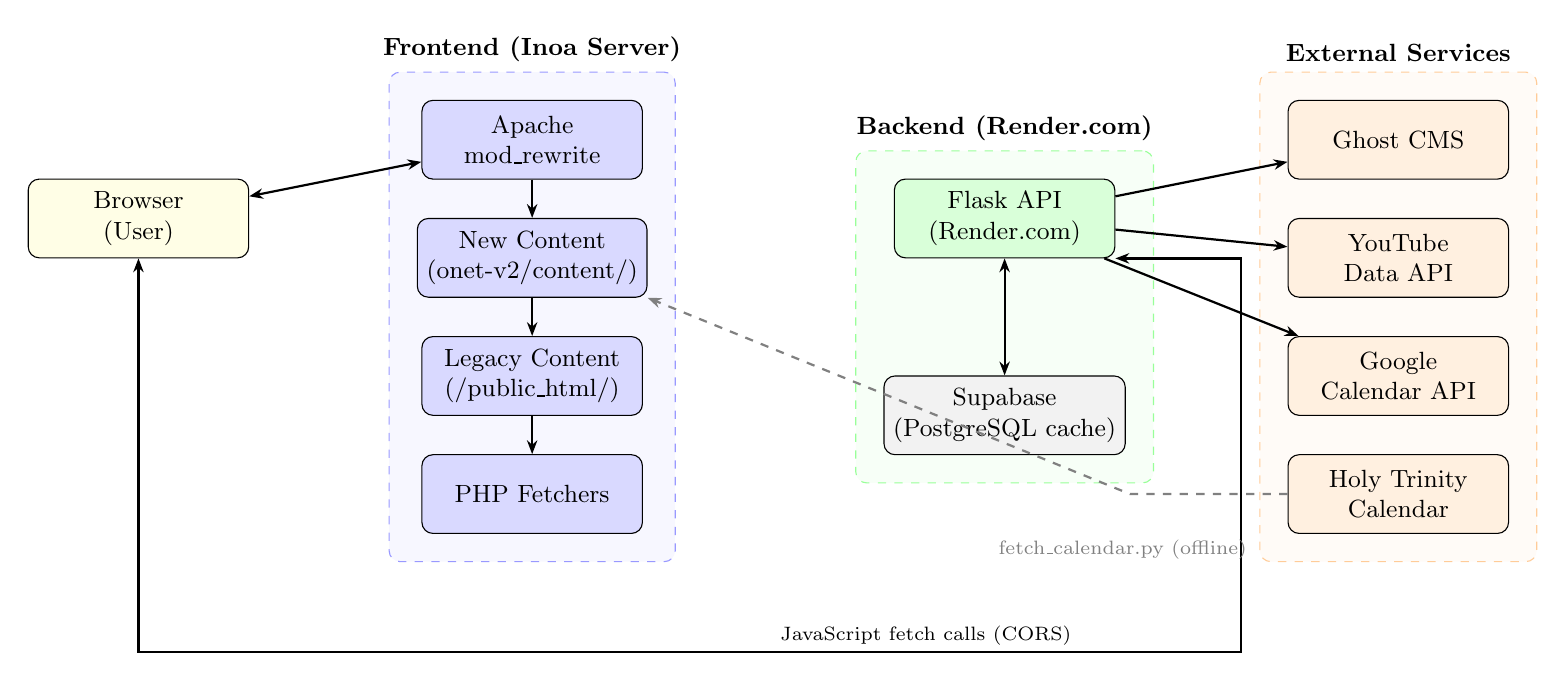
\begin{tikzpicture}[
    box/.style={draw, rounded corners, minimum width=2.8cm, minimum height=1cm, align=center, font=\small},
    frontend/.style={box, fill=blue!15},
    backend/.style={box, fill=green!15},
    external/.style={box, fill=orange!12},
    data/.style={box, fill=gray!10},
    client/.style={box, fill=yellow!10},
    arr/.style={-{Stealth[length=5pt]}, thick},
    darr/.style={{Stealth[length=5pt]}-{Stealth[length=5pt]}, thick},
]

% Client
\node[client] (browser) at (-6, 0) {Browser\\(User)};

% Frontend / Inoa Server
\node[frontend] (apache) at (-1, 1) {Apache\\mod\_rewrite};
\node[frontend] (newcontent) at (-1, -0.5) {New Content\\(onet-v2/content/)};
\node[frontend] (legacy) at (-1, -2) {Legacy Content\\(/public\_html/)};
\node[frontend] (php) at (-1, -3.5) {PHP Fetchers};

% Backend / Render
\node[backend] (flask) at (5, 0) {Flask API\\(Render.com)};
\node[data] (supabase) at (5, -2.5) {Supabase\\(PostgreSQL cache)};

% External Services
\node[external] (ghost) at (10, 1) {Ghost CMS};
\node[external] (youtube) at (10, -0.5) {YouTube\\Data API};
\node[external] (gcal) at (10, -2) {Google\\Calendar API};
\node[external] (holytrin) at (10, -3.5) {Holy Trinity\\Calendar};

% Arrows — browser to frontend
\draw[darr] (browser) -- (apache);
\draw[arr] (apache) -- (newcontent);
\draw[arr] (newcontent) -- (legacy);
\draw[arr] (legacy) -- (php);

% Browser to backend (underneath)
\draw[darr] (browser.south) -- ++(0, -5) -- ++(14, 0) -- ++(0, 5) -- (flask.south east);
\node[font=\scriptsize] at (4, -5.3) {JavaScript fetch calls (CORS)};

% Backend to external
\draw[arr] (flask) -- (ghost);
\draw[arr] (flask) -- (youtube);
\draw[arr] (flask) -- (gcal);

% Backend to cache
\draw[darr] (flask) -- (supabase);

% Holy Trinity to frontend (offline)
\draw[arr, dashed, gray] (holytrin.west) -- +(-2, 0) -- (newcontent.south east);
\node[font=\scriptsize, gray] at (6.5, -4.2) {fetch\_calendar.py (offline)};

% Background groups
\begin{scope}[on background layer]
    \node[draw=blue!40, dashed, fill=blue!3, rounded corners,
        fit=(apache)(newcontent)(legacy)(php),
        inner sep=10pt,
        label={[font=\small\bfseries]above:Frontend (Inoa Server)}] {};
    \node[draw=green!40, dashed, fill=green!3, rounded corners,
        fit=(flask)(supabase),
        inner sep=10pt,
        label={[font=\small\bfseries]above:Backend (Render.com)}] {};
    \node[draw=orange!40, dashed, fill=orange!3, rounded corners,
        fit=(ghost)(youtube)(gcal)(holytrin),
        inner sep=10pt,
        label={[font=\small\bfseries]above:External Services}] {};
\end{scope}

\end{tikzpicture}%
}
\caption{Complete orthodox.net platform architecture.}
\label{fig:platform-arch}
\end{figure}

\subsection{How the Components Interact}

\begin{enumerate}
    \item The \textbf{browser} makes HTTP requests to \texttt{orthodox.net}, which is served by Apache on the Inoa shared hosting server.
    \item Apache's \texttt{.htaccess} routing checks for new content in \texttt{/new/onet-v2/content/} first, falling back to legacy \texttt{/public\_html/} pages.
    \item For legacy content categories (sermons, articles, etc.), Apache rewrites the URL to a \textbf{shell HTML page} that uses JavaScript to fetch content from a \textbf{PHP fetcher script}, which reads and cleans the original legacy HTML file.
    \item For dynamic content (blog posts, videos, calendar), JavaScript in the browser makes direct \textbf{fetch calls to the Flask API} on Render.com (cross-origin, CORS-enabled).
    \item The Flask API aggregates content from \textbf{Ghost CMS} (articles), \textbf{YouTube} (videos), and \textbf{Google Calendar} (services schedule), caching responses in \textbf{Supabase} (PostgreSQL) to reduce API quota usage.
    \item The ``Today's Saints \& Readings'' section uses \textbf{pre-generated static HTML files} scraped from Holy Trinity Orthodox Church's calendar. These are generated offline by a Python script and deployed via git.
\end{enumerate}

%% ============================================================
\section{Technology Stack}
%% ============================================================

\begin{figure}[ht]
\centering
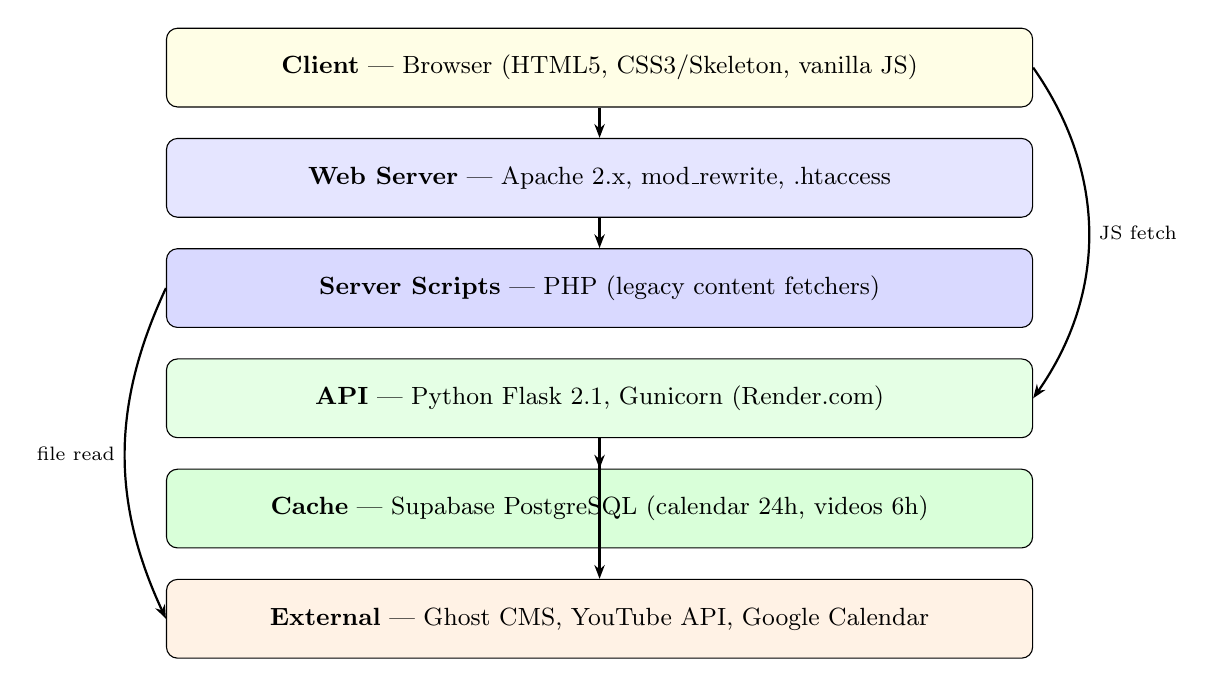
\begin{tikzpicture}[
    layer/.style={draw, rounded corners, minimum width=11cm, minimum height=1cm, align=center, font=\small},
    arr/.style={-{Stealth[length=5pt]}, thick},
]

\node[layer, fill=yellow!10] (client) at (0,0) {\textbf{Client} --- Browser (HTML5, CSS3/Skeleton, vanilla JS)};
\node[layer, fill=blue!10] (server) at (0,-1.4) {\textbf{Web Server} --- Apache 2.x, mod\_rewrite, .htaccess};
\node[layer, fill=blue!15] (php) at (0,-2.8) {\textbf{Server Scripts} --- PHP (legacy content fetchers)};
\node[layer, fill=green!10] (api) at (0,-4.2) {\textbf{API} --- Python Flask 2.1, Gunicorn (Render.com)};
\node[layer, fill=green!15] (cache) at (0,-5.6) {\textbf{Cache} --- Supabase PostgreSQL (calendar 24h, videos 6h)};
\node[layer, fill=orange!10] (ext) at (0,-7.0) {\textbf{External} --- Ghost CMS, YouTube API, Google Calendar};

\draw[arr] (client) -- (server);
\draw[arr] (server) -- (php);
\draw[arr] (client.east) to[bend left=35] node[right, font=\scriptsize] {JS fetch} (api.east);
\draw[arr] (api) -- (cache);
\draw[arr] (api) -- (ext);
\draw[arr] (php.west) to[bend right=25] node[left, font=\scriptsize] {file read} (ext.west);

\end{tikzpicture}
\caption{Technology stack from client to external data sources.}
\label{fig:tech-stack-overview}
\end{figure}

\subsection{Frontend Stack}

\begin{longtable}{p{3.5cm}p{9cm}}
\toprule
\textbf{Technology} & \textbf{Usage} \\
\midrule
HTML5, CSS3 & Markup and styling (Skeleton grid framework, Alegreya font) \\
Vanilla JavaScript & Client-side logic; no frameworks, no build process \\
Apache 2.x & Web server with \texttt{mod\_rewrite} for URL routing \\
PHP & Minimal: content fetcher scripts for legacy migration \\
Python 3 & Utility scripts (template updates, calendar fetching, image conversion) \\
Git & Version control; deployed via \texttt{git pull} on production \\
\bottomrule
\end{longtable}

\subsection{Backend Stack}

\begin{longtable}{p{3.5cm}p{9cm}}
\toprule
\textbf{Technology} & \textbf{Usage} \\
\midrule
Python 3.12 & Core application language \\
Flask 2.1 & Web framework for REST API \\
Gunicorn & WSGI server for production \\
Supabase & PostgreSQL caching layer (calendar events, YouTube videos) \\
Flasgger & Auto-generated Swagger API documentation \\
Render.com & Cloud hosting (staging + production environments) \\
\bottomrule
\end{longtable}

%% ============================================================
\section{External Service Integrations}
%% ============================================================

\begin{figure}[ht]
\centering
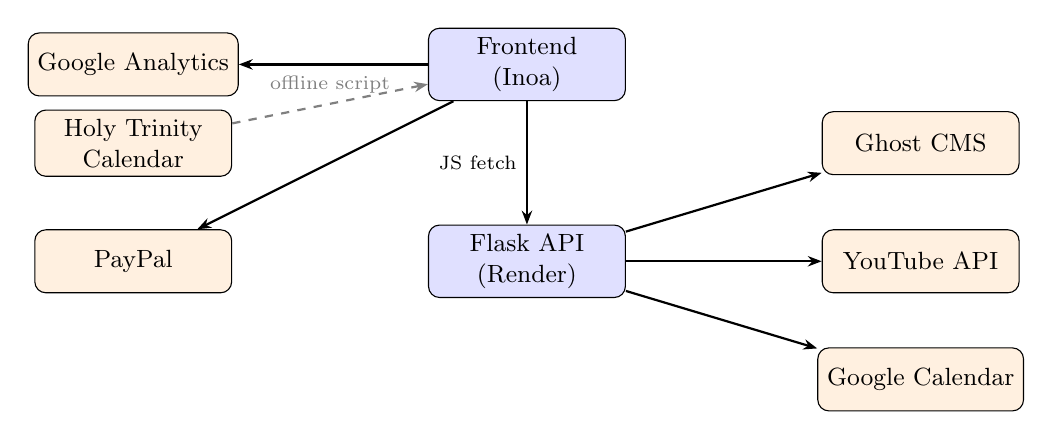
\begin{tikzpicture}[
    svc/.style={draw, rounded corners, minimum width=2.5cm, minimum height=0.8cm, align=center, font=\small, fill=orange!12},
    sys/.style={draw, rounded corners, minimum width=2.5cm, minimum height=0.8cm, align=center, font=\small, fill=blue!12},
    arr/.style={-{Stealth[length=5pt]}, thick},
]

\node[sys] (frontend) at (0, 0) {Frontend\\(Inoa)};
\node[sys] (backend) at (0, -2.5) {Flask API\\(Render)};

\node[svc] (ghost) at (5, -1) {Ghost CMS};
\node[svc] (youtube) at (5, -2.5) {YouTube API};
\node[svc] (gcal) at (5, -4) {Google Calendar};

\node[svc] (htrin) at (-5, -1) {Holy Trinity\\Calendar};
\node[svc] (ga) at (-5, 0) {Google Analytics};
\node[svc] (paypal) at (-5, -2.5) {PayPal};

\draw[arr] (backend) -- (ghost);
\draw[arr] (backend) -- (youtube);
\draw[arr] (backend) -- (gcal);
\draw[arr, dashed, gray] (htrin) -- node[above, font=\scriptsize] {offline script} (frontend);
\draw[arr] (frontend) -- (ga);
\draw[arr] (frontend) -- (paypal);
\draw[arr] (frontend) -- node[left, font=\scriptsize] {JS fetch} (backend);

\end{tikzpicture}
\caption{External service integrations across both components.}
\label{fig:ext-integrations}
\end{figure}

\begin{longtable}{p{3cm}p{3cm}p{6.5cm}}
\toprule
\textbf{Service} & \textbf{Consumed By} & \textbf{Purpose} \\
\midrule
Ghost CMS & Backend API & Headless CMS for articles and blog posts \\
YouTube Data API & Backend API & Video content from \texttt{@orthodoxnet} channel \\
Google Calendar & Backend API & Church services and events schedule \\
Holy Trinity Orthodox & Frontend (offline) & Saints and readings calendar data (pre-generated) \\
Google Analytics & Frontend & Site usage analytics \\
PayPal SDK & Frontend & Donation processing \\
Inoa/OIS & Frontend & Production LAMP hosting (cPanel) \\
Render.com & Backend API & Cloud hosting (staging + production) \\
Supabase & Backend API & PostgreSQL caching layer \\
\bottomrule
\end{longtable}

%% ============================================================
\section{Frontend Summary}
%% ============================================================

The frontend (\texttt{onet-v2}) is a quasi-static website served from a LAMP stack. Key architectural features:

\begin{itemize}
    \item \textbf{Progressive migration}: New pages in \texttt{/new/onet-v2/content/} coexist with legacy pages in \texttt{/public\_html/}. Apache \texttt{.htaccess} rules check new content first and fall back to legacy.
    \item \textbf{Legacy content migration}: 24 content categories are served through shell pages that dynamically load, clean, and re-template legacy HTML via PHP fetcher scripts and JavaScript.
    \item \textbf{No build process}: All files are served directly --- vanilla HTML, CSS, and JavaScript with query-string cache busting.
    \item \textbf{Dynamic content}: Homepage sections (videos, services schedule, blog posts) are populated by JavaScript calling the Flask backend API.
    \item \textbf{Saints \& Readings}: Pre-generated static HTML files from Holy Trinity Orthodox Church, loaded client-side by \texttt{synaxarion.js}. Must be regenerated every 90 days.
    \item \textbf{Deployment}: \texttt{git pull} on the production server via cPanel terminal. The production \texttt{.htaccess} is maintained manually on the server (not deployed via git).
\end{itemize}

For full details, see the frontend technical reference (\texttt{onet\_frontend.pdf}).

%% ============================================================
\section{Backend API Summary}
%% ============================================================

The backend (\texttt{onet-flask-backend}) is a Python Flask REST API that aggregates content from external services. Key architectural features:

\begin{itemize}
    \item \textbf{Single Flask app}: All routes defined in \texttt{app.py}, with integration logic in separate modules (\texttt{fetch\_ghost.py}, \texttt{fetch\_youtube.py}, \texttt{fetch\_calendar.py}).
    \item \textbf{Caching}: Supabase (PostgreSQL) caches calendar events (24-hour TTL) and YouTube videos (6-hour TTL) to reduce API quota usage. Cache misses trigger live API calls with automatic upsert.
    \item \textbf{API documentation}: Interactive Swagger UI at \texttt{/docs} endpoint, auto-generated by Flasgger.
    \item \textbf{Deployment}: Two Render.com Web Services --- production (from \texttt{main} branch) and staging (from \texttt{staging} branch). Auto-deploy on push.
    \item \textbf{CORS}: Open to all origins (\texttt{*}), enabling direct browser-to-API calls from the frontend.
    \item \textbf{No authentication}: All endpoints are public. Admin cache management endpoints are also unauthenticated (known technical debt).
\end{itemize}

\subsection{API Endpoint Summary}

\begin{longtable}{p{4cm}p{8.5cm}}
\toprule
\textbf{Endpoint Group} & \textbf{Key Endpoints} \\
\midrule
Articles (Ghost CMS) & \texttt{/onet\_article\_data}, \texttt{/onet\_article}, \texttt{/article\_by\_slug}, \texttt{/parish\_life}, \texttt{/motd}, \texttt{/legacy\_article} \\
\midrule
Videos (YouTube) & \texttt{/latest\_videos} (cached), \texttt{/homilies\_videos}, \texttt{/childrens\_videos}, \texttt{/catechism\_videos} \\
\midrule
Calendar (Google) & \texttt{/schedule} (cached, next 10 days, US/Central) \\
\midrule
System & \texttt{/heartbeat}, \texttt{/docs} (Swagger UI) \\
\midrule
Admin & \texttt{POST /cache\_videos}, \texttt{/view\_video\_cache} \\
\bottomrule
\end{longtable}

For full endpoint documentation with request/response examples, see the backend technical reference (\texttt{onet\_backend.pdf}).

%% ============================================================
\section{Deployment Overview}
%% ============================================================

\begin{figure}[ht]
\centering
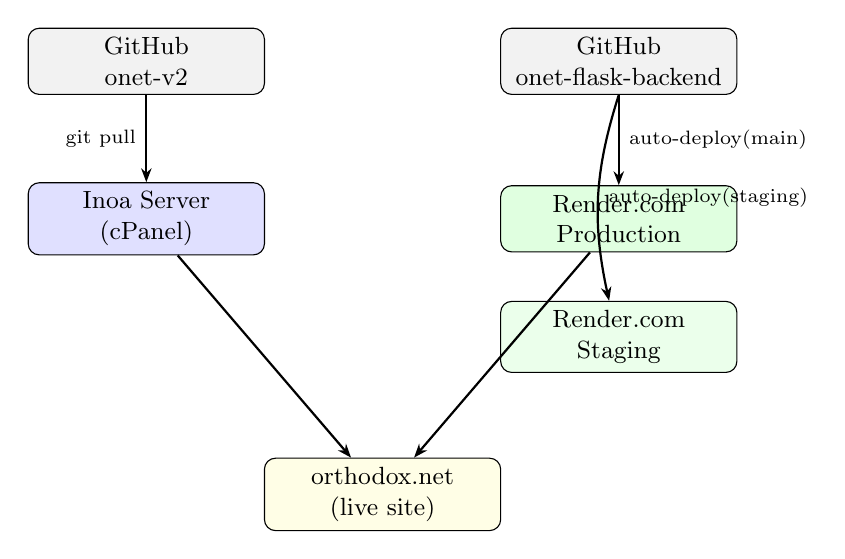
\begin{tikzpicture}[
    box/.style={draw, rounded corners, minimum width=3cm, minimum height=0.8cm, align=center, font=\small},
    arr/.style={-{Stealth[length=5pt]}, thick},
]

% GitHub
\node[box, fill=gray!10] (ghfe) at (-3, 2) {GitHub\\onet-v2};
\node[box, fill=gray!10] (ghbe) at (3, 2) {GitHub\\onet-flask-backend};

% Deployment targets
\node[box, fill=blue!12] (inoa) at (-3, 0) {Inoa Server\\(cPanel)};
\node[box, fill=green!12] (renderprod) at (3, 0) {Render.com\\Production};
\node[box, fill=green!8] (renderstag) at (3, -1.5) {Render.com\\Staging};

% Live site
\node[box, fill=yellow!10] (site) at (0, -3.5) {orthodox.net\\(live site)};

% Arrows
\draw[arr] (ghfe) -- node[left, font=\scriptsize] {git pull} (inoa);
\draw[arr] (ghbe) -- node[right, font=\scriptsize] {auto-deploy\\(main)} (renderprod);
\draw[arr] (ghbe.south) to[bend right=15] node[right, font=\scriptsize] {auto-deploy\\(staging)} (renderstag);
\draw[arr] (inoa) -- (site);
\draw[arr] (renderprod) -- (site);

\end{tikzpicture}
\caption{Deployment pipeline for both components.}
\label{fig:deploy-overview}
\end{figure}

\begin{longtable}{p{3cm}p{3.5cm}p{6cm}}
\toprule
\textbf{Component} & \textbf{Hosting} & \textbf{Deployment Method} \\
\midrule
Frontend & Inoa/OIS (cPanel) & Manual \texttt{git pull} via cPanel terminal \\
Backend (prod) & Render.com & Auto-deploy on push to \texttt{main} branch \\
Backend (staging) & Render.com & Auto-deploy on push to \texttt{staging} branch \\
\bottomrule
\end{longtable}

\textbf{Important}: The frontend's production \texttt{.htaccess} at \texttt{\textasciitilde/public\_html/.htaccess} is \emph{not} deployed via \texttt{git pull}. It must be maintained manually on the server. See the frontend technical reference for details.

%% ============================================================
\section{Key URLs}
%% ============================================================

\begin{longtable}{p{3.5cm}p{9cm}}
\toprule
\textbf{Resource} & \textbf{URL} \\
\midrule
Live site & \url{https://www.orthodox.net} \\
Frontend repo & \url{https://github.com/GZancewicz/onet-v2} \\
Backend repo & \url{https://github.com/GZancewicz/onet-flask-backend} \\
API (production) & \url{https://production-orthodox-net-flask.onrender.com} \\
API (staging) & \url{https://staging-orthodox-net-flask.onrender.com} \\
API docs (Swagger) & \url{https://production-orthodox-net-flask.onrender.com/docs} \\
API health check & \url{https://production-orthodox-net-flask.onrender.com/heartbeat} \\
\bottomrule
\end{longtable}

%% ============================================================
\section{Credentials and Access}
%% ============================================================

To maintain the platform, you need access to:

\begin{enumerate}
    \item \textbf{GitHub}: Write access to both repositories
    \item \textbf{Inoa/OIS cPanel}: Hosting control panel (file manager, terminal, PHP config)
    \item \textbf{Render.com}: Dashboard for backend deployment (environment variables, logs, manual deploys)
    \item \textbf{Ghost CMS}: Admin login for article/post management
    \item \textbf{Google Cloud}: API keys for YouTube Data API and Google Calendar API
    \item \textbf{Supabase}: Project dashboard for database management
    \item \textbf{Google Analytics}: Access to property \texttt{G-D9YEGT19W7}
    \item \textbf{PayPal}: Business account for donation configuration
    \item \textbf{DNS}: Managed by Inoa/OIS
\end{enumerate}

\textbf{Known issue}: Ghost CMS API key and YouTube API key are currently hardcoded in the backend source code rather than read from environment variables. See the backend technical reference for details on this technical debt.

%% ============================================================
\section{Periodic Maintenance}
%% ============================================================

\begin{longtable}{p{3.5cm}p{3cm}p{6cm}}
\toprule
\textbf{Task} & \textbf{Frequency} & \textbf{Details} \\
\midrule
Calendar data refresh & Every 90 days & Run \texttt{fetch\_calendar.py} to regenerate saints/readings HTML files. Run locally and on server. \\
\midrule
Backend monitoring & As needed & Check \texttt{/heartbeat}. Render free-tier services may sleep after inactivity. \\
\midrule
API quota monitoring & Monthly & YouTube Data API has daily quota limits. Caching reduces usage but monitor via Google Cloud console. \\
\midrule
SSL certificates & Automatic & Inoa and Render both handle SSL renewal automatically. \\
\midrule
Production .htaccess & On routing changes & Must be updated manually on server when adding new legacy folder conversions. \\
\bottomrule
\end{longtable}

\end{document}
